\section{Introductory example: dispatch on special matrix types}

\paragraph{Special matrix types}
As befits a language for technical computing, the Julia base library defines
many specializes matrix types which capture information about matrix properties
such as triangularity, Hermitianness or bandedness. Knowing these matrix
properties allows for many efficient computations on them, as many specialized
linear algebra algorithms exist that take advantage of such information.
Furthermore some matrix properties lend themselves to multiple representations.
For example, symmetric matrices may be stored as ordinary matrices, but only
the upper or lower half is ever accessed. Alternatively, they may be stored in
other ways, such as the packed format or rectangular full packed format, which
allow for some faster algorithms, for example, for the Cholesky
factorization~\cite{Gustavson2010}. All three storage formats for symmetric
matrices exist in the LAPACK library for numerical linear algebra; computations
on these formats are distinguished by whether the second and third letters of
the routine's name are \lstinline|SY|, \lstinline|SP| or \lstinline|SF|
respectively. In contrast, Julia's base library contains types like
\lstinline|Symmetric| and \lstinline|SymmetricRFP|, which encode information
about matrix properties and their storage format.

\paragraph{The matrix square root}
Having matrix types like \lstinline|Symmetric| allows Julia programmers to
write code that annotates if a matrix is symmetric. Sometimes, users
will use only symmetric matrices, for example, in code that
works only on adjacency matrices of undirected graphs. In such situations,
it is sensible to construct \lstinline|Symmetric| matrices explictly, as then
Julia can dispatch directly onto specialized methods for \lstinline|Symmetric|
types. An example of such a function is \lstinline|sqrtm|, which computes the
principal square root of a matrix. In general, the square root can be computed
via the Schur factorization of a matrix~\cite{Golub2013}. However, the square
root of a \lstinline|Symmetric| matrix can be computed faster and more stably
by diagonalization to find its eigenvalues and
eigenvectors~\cite{Higham2008,Golub2013}. Hence, it is always advantageous to
use the spectral factorization method for \lstinline|Symmetric| matrices.

Here is a simple example:
%
\begin{lstlisting}
A = Symmetric([1 0 0; 0 0 1; 0 1 0])
B = sqrtm(A)
println(norm(B^2 - A))
\end{lstlisting}
%
$A$ is the adjacency matrix of a graph with 3 vertices and 2 edges, 1--1 and
2--3. \lstinline|Symmetric(...)| constructs a \lstinline|Symmetric| matrix
which wraps the underlying ordinary two-dimensional matrix (of
\lstinline|Matrix| type in Julia). The last line computes the matrix 2-norm
between the square of $B$ and the original matrix $A$ and prints the result to
the standard output stream. In exact arithmetic, the answer would be 0 exactly,
but the actual norm will in general be nonzero due to floating point roundoff.

\paragraph{Dynamic dispatch}
Of course, \lstinline|sqrtm| can be used in more general situations where the
input matrix may not have any known symmetries and may simply be an ordinary
\lstinline|Matrix|. Without any further information, the only choice is the
more expensive algorithm that uses the Schur factorization. However, the speed
and stability of the specialized method suggests an advantage from checking if
the input \lstinline|Matrix| is symmetric at run time, and if so, dispatching
onto the method defined for \lstinline|Symmetric| inputs instead. This is
exactly what Julia's implementation of \lstinline|sqrtm| does:\footnote{
The code listing is taken directly from the Julia base library, with minor
changes for clarity.}
%
\begin{lstlisting}
function sqrtm{T<:Real}(A::StridedMatrix{T})
    #If symmetric, use specialized method
    issym(A) && return sqrtm(Symmetric(A))

    #Otherwise, use general method
    SchurF = schurfact(complex(A))
    R = full(sqrtm(Triangular(SchurF[:T], :U, false)))
    retmat = SchurF[:vectors]*R*SchurF[:vectors]'

    #If result has no imaginary component, return a matrix of real numbers
    all(imag(retmat) .== 0) ? real(retmat) : retmat
end
\end{lstlisting}

Figure~\ref{fig:sqrtm} summarizes the high level behavior of \lstinline|sqrtm|.
The general method first checks if the input matrix is symmetric, which is fast
compared to the actual computation of the square root. If the matrix is found to
be symmetric, it is wrapped in a \lstinline|Symmetric| constructor, which allows
Julia to dispatch onto the specialized method. Otherwise, the next few lines
computes the square root. Thus dynamic dispatch allows the same performant
kernel to be called even in situations where the user does not know if a
particular input matrix is symmetric, or even that specialized algorithms for
symmetric matrices exist.

The first code snippet illustrates a situation that can be addressed by either
static dispatch or dynamic dispatch. However, the second snippet makes use of
dynamic dispatch semantics to reuse code for the special case, if at run time
the input was determined to satisfy the conditions of the special case. If we
only had static dispatch semantics, then we either have to forgo the
specialized algorithm, or otherwise repeat that code in the general method.
Therefore, dynamic dispatch allows for greater code reuse, allowing for greater
overall performance without redundant code.



\subsection{Polymorphic types in Julia}

The method shown above also demonstrates two kinds of polymorphism supported in
Julia. First, the input \lstinline|A| is annotated (\lstinline|::|) with the
type \lstinline|StridedMatrix|, which is an abstract type, not a concrete type.
A strided matrix is one that has a Fortran-compatible storage format, i.e.\ it
is stored in a contiguous block of memory and whose dimensions can be described
by a dope vector. The subtypes of \lstinline|StridedMatrix| in the base
library are \lstinline|Matrix| (ordinary matrices), and subarray types defining
views into strided matrices, whose referenced elements may not be fully
contiguous in memory. Thus, this \lstinline|sqrtm| method would be
dispatched upon by both \lstinline|Matrix| objects and subarrays, by virtue of
both types being subtypes of \lstinline|StridedMatrix|.

The second kind of polymorphism shown by the signature
\lstinline|sqrtm{T<:Real}(A::Matrix{T})| is parametric polymorphism. This
signature defines a family of related methods, one for each kind of
\lstinline|Matrix| containing a numeric type \lstinline|T| that is a subtype
(\lstinline|<:|) of \lstinline|Real|. This definition encompasses separate
definitions for matrices of type \lstinline|Matrix{Int32}| (matrices of 32-bit
integers), \lstinline|Matrix{Float64}| (matrices of 64-bit floating point real
numbers), and even \lstinline|Matrix{Rational{BigInt}}| (matrices of rational
numbers where the numerators and denominators are arbitrary precision
integers). Matrices containing other types, such as
\lstinline|Matrix{Complex{Float64}}|, would not dispatch on this family of methods.

The two kinds of polymorphism allow families of related methods to be defined
concisely, which allow highly generic code to be written. Additionally, code for
multiple algorithms can coexist within the same generic function, with the actual
choice of which code to run being determined by method dispatch.



\subsection{Dynamic dispatch in matrix functions}

Dynamic, i.e.\ late bound, dispatch allows for high performance
polyalgorithms with specialized code paths depending on matrix properties which
can only be inferred at runtime based on the specific values of the inputs. For
example, the matrix square root (\verb|sqrtm|) has two methods defined:

\begin{itemize}
	\item For symmetric (or Hermitian) matrices, where the answer can be
		computed by diagonalization,
	\item For general dense matrices, where the answer uses the more
		expensive (but also more general) Schur
		factorization~\cite{Higham2008}.
\end{itemize}
%
The latter method contains a run time check for symmetry and dispatches upon
the former if present. Thus as summarized in Figure~\ref{fig:sqrtm}, dynamic
dispatch allows the same performant kernel to be called even in situations
where the user does not know if a particular input matrix is symmetric, or even
that specialized algorithms for symmetric matrices exist.


\begin{lstlisting}
function sqrtm{T<:Real}(A::StridedMatrix{T})
    issym(A) && return sqrtm(Symmetric(A))
    n = chksquare(A)
    SchurF = schurfact(complex(A))
    R = full(sqrtm(Triangular(SchurF[:T], :U, false)))
    retmat = SchurF[:vectors]*R*SchurF[:vectors]'
    all(imag(retmat) .== 0) ? real(retmat) : retmat
end
\end{lstlisting}


\begin{figure}
	\centering
	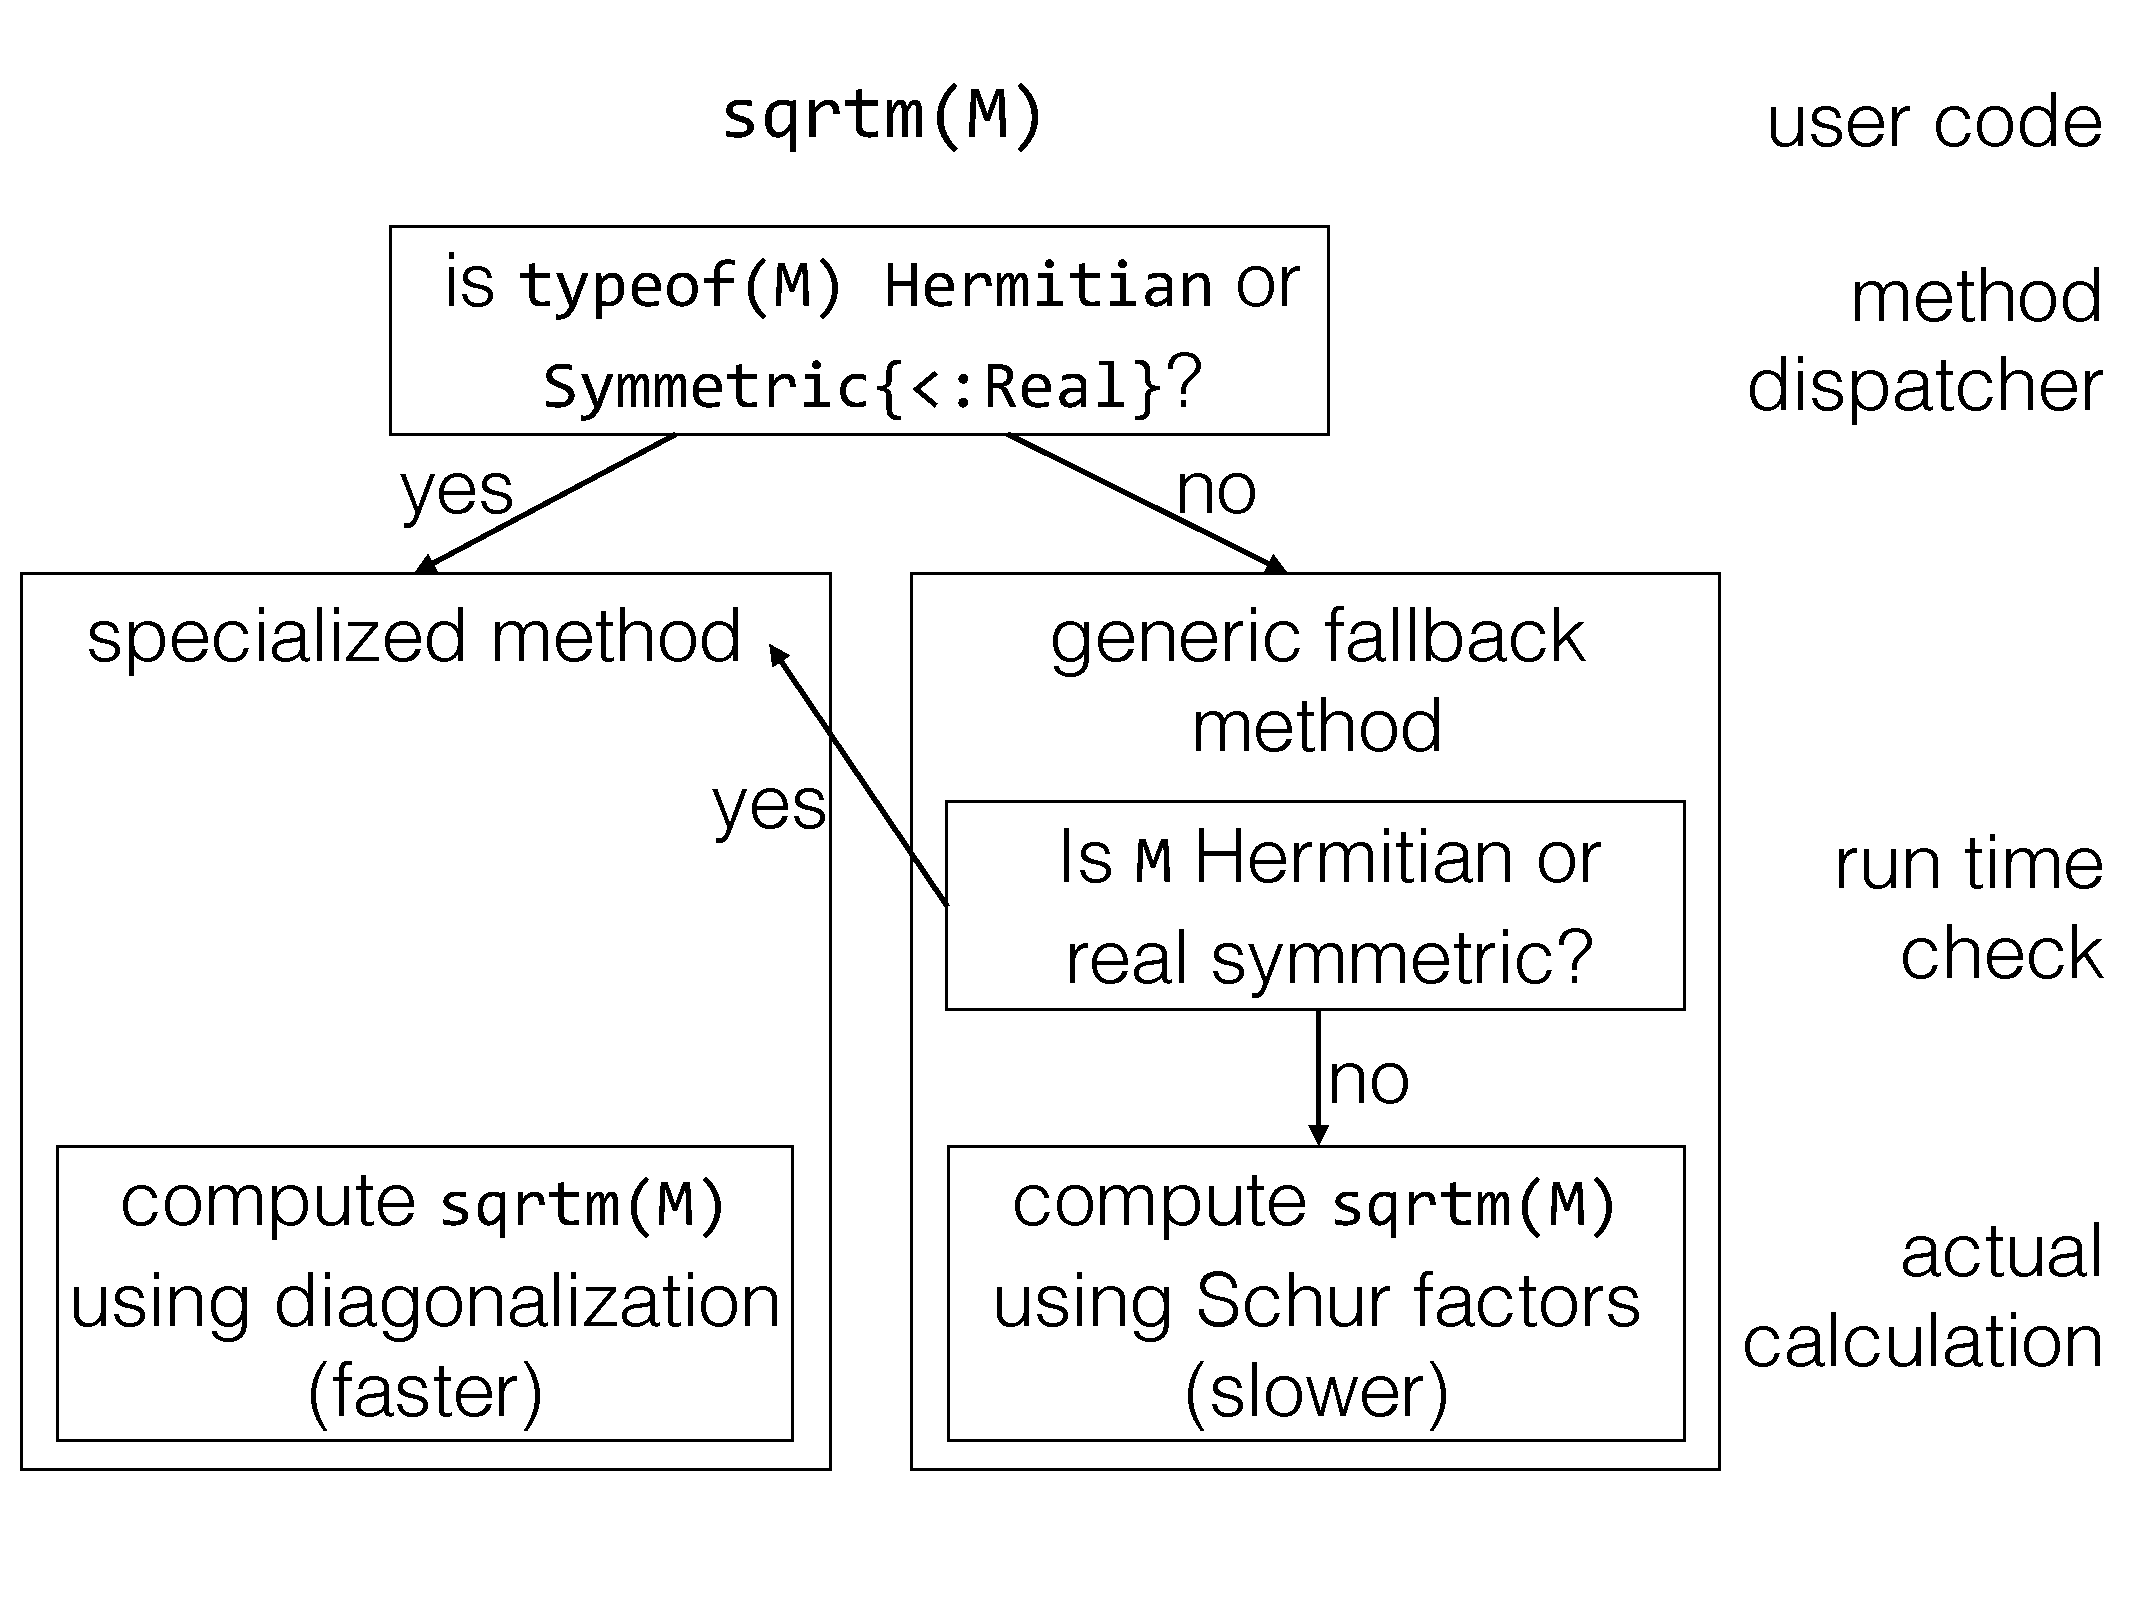
\includegraphics[width=\columnwidth]{fig-sqrtm}
	\caption{Dynamic dispatch and multimethods for the matrix square root
		function \texttt{sqrtm}, showing that the specialized algorithm
		can be run either from a static decision from the method
		dispatcher based on the input type, or a dynamic decision from
		a run-time check based on the value.}
	\label{fig:sqrtm}
\end{figure}




\subsection{Late binding increases expressiveness}

The examples in this section, while simple, illustrate the expressive power
afforded by the composition of extensible generic functions, polymorphic types,
dynamic multiple dispatch, and aggressive method specialization allowed by
just-in-time static analyses. Users are allowed to extend both the collection
of generic functions and the base type hierarchy in Julia, which further erodes
the distinction between user code and library code that is itself written in
Julia. We believe that such expressivity is useful for technical computing
applications, where it is not generally possible to predict the variety of
specialized computations that domain scientists, engineeers and mathematicians
require.

Some other languages also offer constructs for type polymorphism, like C++'s
expression templates and Fortress's generic functions, but these constructs are
only available at compile time, which restrict their expressiveness.
Furthermore, these languages usually require that all possible specialized
methods be generated at compile time, resulting in long compilation times which
are curtailed in practice with further restrictions on the generality of user
defined code. In contrast, the combination of dynamic multiple dispatch
semantics and on-demand method specialization in Julia allows users to write
highly generic code. Consider that the method definitions above each represent
an infinite family of methods. While user code in practice only uses a small,
finite subset of the possible methods, users have the luxury of choosing from
the entire universe encompassed by the generic function system.

